%!TEX root = thesis.tex


\begin{figure}
\centering
                        \scalebox{1.0}{
                            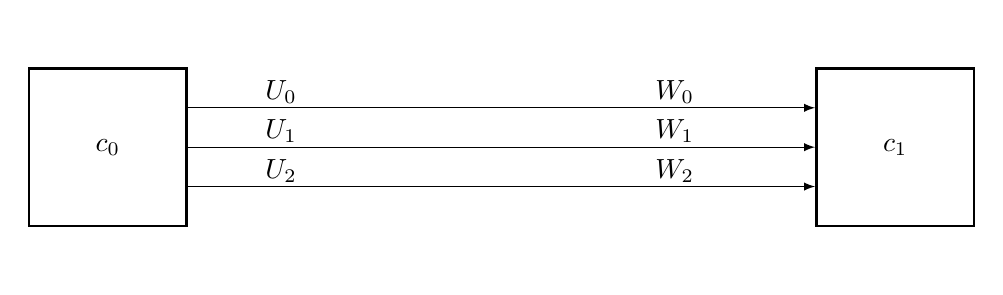
\begin{tikzpicture}
                                [
                                    square/.style = {draw, shape=rectangle, minimum height=2cm, minimum width=2cm, node distance=2cm, line width=1pt},
                                    empty/.style = {draw, shape=rectangle, minimum height=2cm, minimum width=2cm, node distance=2cm, line width=1pt, draw=white},
                                ]

                                \node[empty] (0a) at (0,0.5)     {};
                                \node[empty] (0b) at (0,-0.5)     {};
                                \node[square] (0c) at (0,0)     {$c_0$};

                                \node[empty] (1a) at (10cm,0.5)   {};
                                \node[empty] (1b) at (10cm,-0.5)   {};
                                \node[square] (1c) at (10cm,0)   {$c_1$};

                                \node (x0) at (2.2cm,0.7) {$U_0$};
                                \node (y0) at (2.2cm,-0.3) {$U_2$};
                                \node (z0) at (2.2cm,0.2) {$U_1$};

                                \node (x1) at (7.2cm,0.7) {$W_0$};
                                \node (y1) at (7.2cm,-0.3) {$W_2$};
                                \node (z1) at (7.2cm,0.2) {$W_1$};

                                \draw [-latex] (0a.east) -- (1a.west);
                                \draw [-latex] (0b.east) -- (1b.west);
                                \draw [-latex] (0c.east) -- (1c.west);
                            \end{tikzpicture}
                            
                        }
                        \caption{An example of linking component $c_0$ to component $c_1$. The output wires of $c_1$, $U_0, U_1$ and $U_2$, are linked to the input wires of $c_1$, $W_0, W_1$ and $W_2$.}
                            \label{fig:chaining}
                    \end{figure}
                    
                    
                    %!TEX root = thesis.tex
%
%
%\begin{figure}
%\centering
%                        \scalebox{1.0}{
%                            \begin{tikzpicture}
%                                [
%                                    square/.style = {draw, shape=rectangle, minimum height=2cm, minimum width=2cm, node distance=2cm, line width=1pt},
%                                    empty/.style = {draw, shape=rectangle, minimum height=2cm, minimum width=2cm, node distance=2cm, line width=1pt, draw=white},
%                                ]
%
%                                \node[empty] (0a) at (0,0.5)     {};
%                                \node[empty] (0b) at (0,-0.5)     {};
%                                \node[square] (0c) at (0,0)     {$c_0$};
%
%                                \node[color=blue] (mida) at (4.8cm,0.5)   {$A \oplus X$};
%                                \node[color=blue] (midb) at (4.8cm,-0.5)  {$C \oplus Z$}; 
%                                \node[color=blue] (midc) at (4.8cm,0)     {$B \oplus Y$};
%
%                                \node[empty] (1a) at (10cm,0.5)   {};
%                                \node[empty] (1b) at (10cm,-0.5)   {};
%                                \node[square] (1c) at (10cm,0)   {$c_1$};
%
%                                \node (x0) at (2.2cm,0.7) {$U_0$};
%                                \node (y0) at (2.2cm,-0.3) {$U_2$};
%                                \node (z0) at (2.2cm,0.2) {$U_1$};
%
%                                \node (x1) at (7.2cm,0.7) {$W_0$};
%                                \node (y1) at (7.2cm,-0.3) {$W_2$};
%                                \node (z1) at (7.2cm,0.2) {$W_1$};
%
%                                \draw [-latex] (0a.east) -- (mida.west);
%                                \draw [-latex] (0b.east) -- (midb.west);
%                                \draw [-latex] (0c.east) -- (midc.west);
%
%                                \draw [-latex] (mida.east) -- (1a.west);
%                                \draw [-latex] (midb.east) -- (1b.west);
%                                \draw [-latex] (midc.east) -- (1c.west);
%                            \end{tikzpicture}
%                        }
%                    \end{figure}